%********************************************************************
% Kapitel 4: Konzeption
%********************************************************************
\chapter{Konzeption}
\label{ch:konzeption}

Dieses Kapitel beschreibt die Konzeption der entwickelten Monitoring-Lösung. Aufbauend auf den in Kapitel~\ref{ch:analyse} ermittelten Anforderungen und den identifizierten Lücken werden eigene Lösungsansätze vorgestellt, die diese Lücken schließen und die Anforderungen erfüllen. Die Konzeption erfolgt technologieunabhängig, das heißt, die beschriebenen Konzepte und Architekturen sind unabhängig von konkreten Implementierungstechnologien wie Java, Spring Boot oder Prometheus formuliert.

\section{Überblick über die Gesamtarchitektur}
\label{sec:gesamtarchitektur}

Die entwickelte Lösung folgt einer modularen Architektur, die aus mehreren miteinander verbundenen Komponenten besteht. Die Architektur orientiert sich an etablierten Prinzipien der Softwarearchitektur, insbesondere am Separation-of-Concerns-Prinzip und an der Schichtenarchitektur \cite{software-architecture-patterns}. Abbildung~\ref{fig:architekturuebersicht} zeigt eine konzeptionelle Übersicht der Gesamtarchitektur.

\begin{figure}[h]
\centering
% TODO: Architekturdiagramm einfügen (z.B. als PDF oder PNG)
\IfFileExists{Chapters/Graphics/architekturuebersicht.drawio.png}{%
    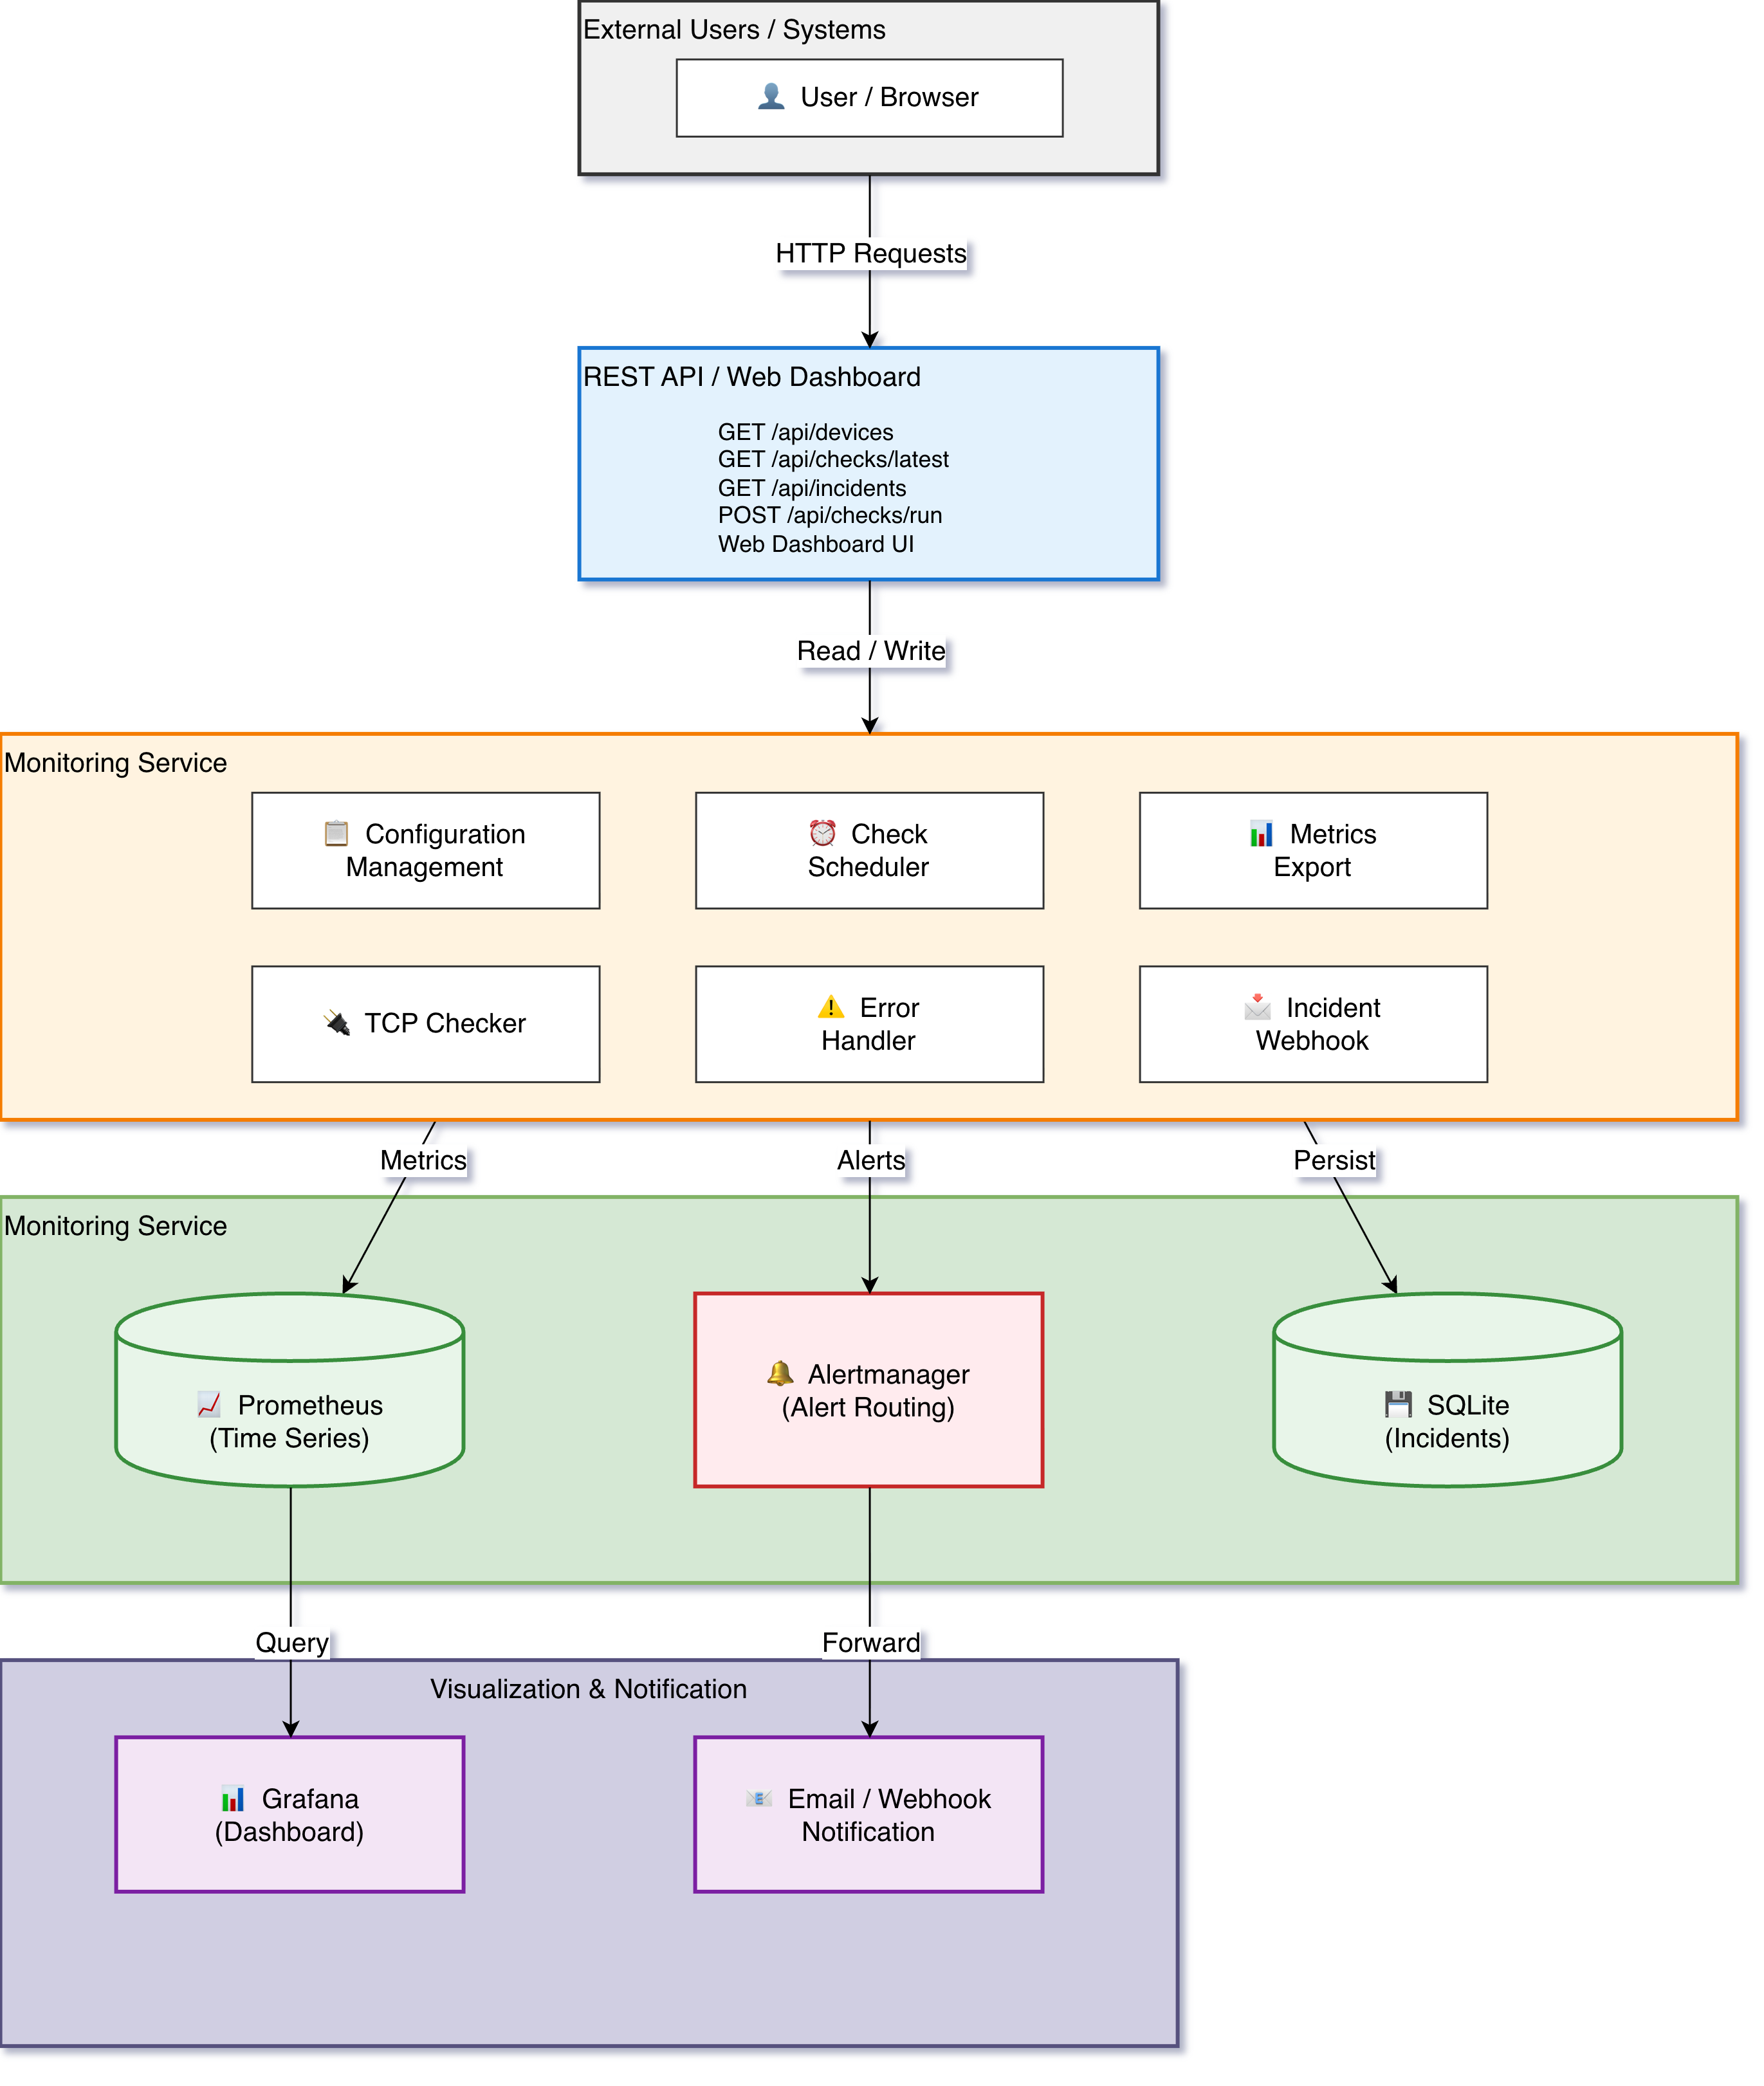
\includegraphics[width=0.8\textwidth]{Chapters/Graphics/architekturuebersicht.drawio.png}
}{%
    \fbox{\parbox[c][4cm][c]{0.8\textwidth}{\centering Architekturdiagramm fehlt\newline (Datei nicht gefunden)}}
}
\caption{Konzeptionelle Übersicht der Gesamtarchitektur}
\label{fig:architekturuebersicht}
\end{figure}

Die Architektur umfasst folgende Hauptkomponenten:

\begin{itemize}
    \item \textbf{Monitoring-Dienst:} Zentrale Komponente zur Verwaltung der Überwachungsziele und Ausführung der Erreichbarkeitsprüfungen.
    \item \textbf{Metrik-Export:} Bereitstellung der Prüfergebnisse in einem standardisierten Format für externe Monitoring-Systeme.
    \item \textbf{Zeitreihenspeicher:} Persistierung der Metriken als Zeitreihen für aktuelle und historische Auswertungen.
    \item \textbf{Visualisierung:} Darstellung der Metriken und Zustände in Dashboards.
    \item \textbf{Alert-Komponente:} Erkennung kritischer Zustände und Weiterleitung von Benachrichtigungen.
    \item \textbf{Incident-Speicher:} Persistente Speicherung von Alerts als Incidents zur langfristigen Nachverfolgung.
    \item \textbf{REST-Schnittstelle:} Operative Abfrage von Konfiguration, Prüfergebnissen und Incidents.
\end{itemize}

Die Komponenten kommunizieren über definierte Schnittstellen miteinander. Der Monitoring-Dienst führt die Prüfungen durch und stellt die Ergebnisse über den Metrik-Export bereit. Der Zeitreihenspeicher ruft die Metriken regelmäßig ab und speichert sie. Die Visualisierungskomponente greift auf den Zeitreihenspeicher zu, um Dashboards zu erstellen. Die Alert-Komponente wertet die gespeicherten Metriken aus und leitet bei kritischen Zuständen Benachrichtigungen an den Incident-Speicher weiter.

\section{Schließen der identifizierten Lücken}
\label{sec:schliessen-der-luecken}

Die Konzeption adressiert explizit die in Abschnitt~\ref{subsec:abdeckungsanalyse} identifizierten Lücken bestehender Monitoring-Lösungen. Die Lösungsansätze orientieren sich an bewährten Praktiken aus Forschung und Industrie \cite{requirements-engineering-best-practices}.

\subsection{Lücke 1: Fehlende Incident-Historie}
\label{subsec:loesung-luecke-1}

Um die fehlende Incident-Historie bestehender Lösungen zu adressieren, wird eine eigene Komponente zur persistenten Speicherung von Incidents konzipiert. Jedes Incident umfasst folgende Informationen:

\begin{itemize}
    \item Eindeutige Identifikation (z.B. Fingerprint des Alerts)
    \item Alert-Name und Beschreibung
    \item Betroffenes Gerät (Name, Host, Port)
    \item Schweregrad (z.B. Warning, Critical)
    \item Status (Firing oder Resolved)
    \item Startzeitpunkt und optionaler Auflösungszeitpunkt
    \item Zusammenfassung und detaillierte Beschreibung
\end{itemize}

Die Incident-Historie ermöglicht die langfristige Nachverfolgung von Störungen unabhängig von der Zeitreihen-Retention des Monitoring-Systems. Durch die Speicherung von Start- und Auflösungszeitpunkt kann die Dauer jeder Störung berechnet und analysiert werden. Dieses Konzept orientiert sich an etablierten Incident-Management-Praktiken \cite{incident-management-itil}.

\subsection{Lücke 2: Fehlende integrierte REST-Schnittstelle}
\label{subsec:loesung-luecke-2}

Um eine umfassende REST-Schnittstelle bereitzustellen, wird eine API-Komponente konzipiert, die folgende Endpunkte bereitstellt:

\begin{itemize}
    \item Abfrage der konfigurierten Überwachungsziele
    \item Abfrage der aktuellen Prüfergebnisse
    \item Abfrage der historischen Prüfergebnisse mit Filtermöglichkeiten
    \item Abfrage aller Incidents und der aktiven Incidents
    \item Abfrage des Dienststatus
    \item Manuelle Auslösung eines Prüfzyklus
    \item Empfang von Alert-Webhooks
\end{itemize}

Die REST-Schnittstelle ermöglicht die Integration mit externen Systemen und die automatisierte Abfrage von Monitoring-Daten. Administrative Endpunkte werden durch Authentifizierung und Autorisierung geschützt. Die API-Design-Entscheidungen orientieren sich an den Prinzipien des REST-Architekturstils \cite{rest-architectural-style}.

\subsection{Lücke 3: Komplexe Bereitstellung}
\label{subsec:loesung-luecke-3}

Um die Bereitstellung zu vereinfachen, wird die gesamte Monitoring-Umgebung als containerisierte Anwendung konzipiert. Alle Komponenten werden in separaten Containern ausgeführt und über ein gemeinsames Netzwerk verbunden. Die Konfiguration erfolgt über eine zentrale Konfigurationsdatei, die alle Services, Netzwerke und Volumes definiert.

Diese Konzeption ermöglicht:

\begin{itemize}
    \item Einheitlichen Start aller Komponenten mit einem Befehl
    \item Reproduzierbare Bereitstellung in verschiedenen Umgebungen
    \item Einfache Skalierung und Wartung einzelner Komponenten
    \item Isolierte Ausführung mit definierten Ressourcenkontingenten
\end{itemize}

Die Containerisierung folgt etablierten Best Practices für containerisierte Anwendungen \cite{docker-best-practices}.

\subsection{Lücke 4: Überdimensionierung}
\label{subsec:loesung-luecke-4}

Um Überdimensionierung zu vermeiden, wird die Lösung bewusst schlank gehalten und konzentriert sich auf die Kernfunktionen:

\begin{itemize}
    \item TCP-basierte Erreichbarkeitsprüfungen
    \item Metrik-Export für externe Monitoring-Systeme
    \item Visualisierung über externe Dashboards
    \item Incident-Management mit persistenter Historie
    \item REST-API für operative Abfragen
\end{itemize}

Komplexe Funktionen wie automatische Discovery, umfassende Plugin-Systeme oder Enterprise-Features werden bewusst nicht implementiert, um die Leichtgewichtigkeit zu erhalten. Dieses Vorgehen orientiert sich am Prinzip der minimalen Funktionalität (Minimal Viable Product) \cite{lean-software-development}.

\subsection{Lücke 5: Fehlende manuelle Auslösung}
\label{subsec:loesung-luecke-5}

Um die manuelle Auslösung von Prüfzyklen zu ermöglichen, wird ein dedizierter Endpunkt konzipiert, der bei Aufruf einen sofortigen Prüfzyklus für alle aktivierten Ziele startet. Diese Funktion unterstützt Tests, Fehlersuche und Demonstrationen, da ein neuer Zustand gezielt erzeugt und unmittelbar überprüft werden kann.

\section{Konzeption des Monitoring-Dienstes}
\label{sec:konzeption-monitoring-dienst}

Der Monitoring-Dienst bildet die zentrale Komponente der Lösung. Er übernimmt die Verwaltung der Überwachungsziele, die Ausführung der Prüfungen und die Bereitstellung der Ergebnisse.

\subsection{Verwaltung der Überwachungsziele}
\label{subsec:verwaltung-ueberwachungsziele}

Die Überwachungsziele werden in einer Konfigurationsdatei verwaltet. Jedes Ziel umfasst folgende Attribute:

\begin{itemize}
    \item \textbf{Identifikation:} Eindeutige ID und lesbarer Name
    \item \textbf{Zieladresse:} Hostname oder IP-Adresse
    \item \textbf{Port:} Zu prüfender TCP-Port
    \item \textbf{Aktivierungsstatus:} Gibt an, ob das Ziel aktiv überwacht wird
\end{itemize}

Zusätzlich werden globale Parameter definiert:

\begin{itemize}
    \item \textbf{Prüfintervall:} Zeit zwischen zwei Prüfzyklen
    \item \textbf{Timeout:} Maximale Wartezeit für einen Verbindungsversuch
    \item \textbf{Historien-Retention:} Speicherdauer für Prüfergebnisse und Incidents
\end{itemize}

Diese Trennung von Konfiguration und Fachlogik ermöglicht die Anpassung der Überwachungsziele ohne Änderungen am Quellcode (Anforderung N1). Dieses Konzept folgt dem Prinzip der Externalisierung von Konfigurationen \cite{configuration-management-patterns}.

\subsection{Ausführung der Erreichbarkeitsprüfungen}
\label{subsec:ausfuehrung-pruefungen}

Die Prüfungen erfolgen nach dem Prinzip des zeitgesteuerten Pollings. In regelmäßigen Intervallen wird für jedes aktivierte Ziel versucht, eine TCP-Verbindung zum konfigurierten Host und Port aufzubauen.

Abbildung~\ref{fig:pruefablauf} zeigt den Ablauf einer einzelnen Prüfung.

\begin{figure}[h]
\centering
% TODO: Flussdiagramm einfügen (z.B. als PDF oder PNG)
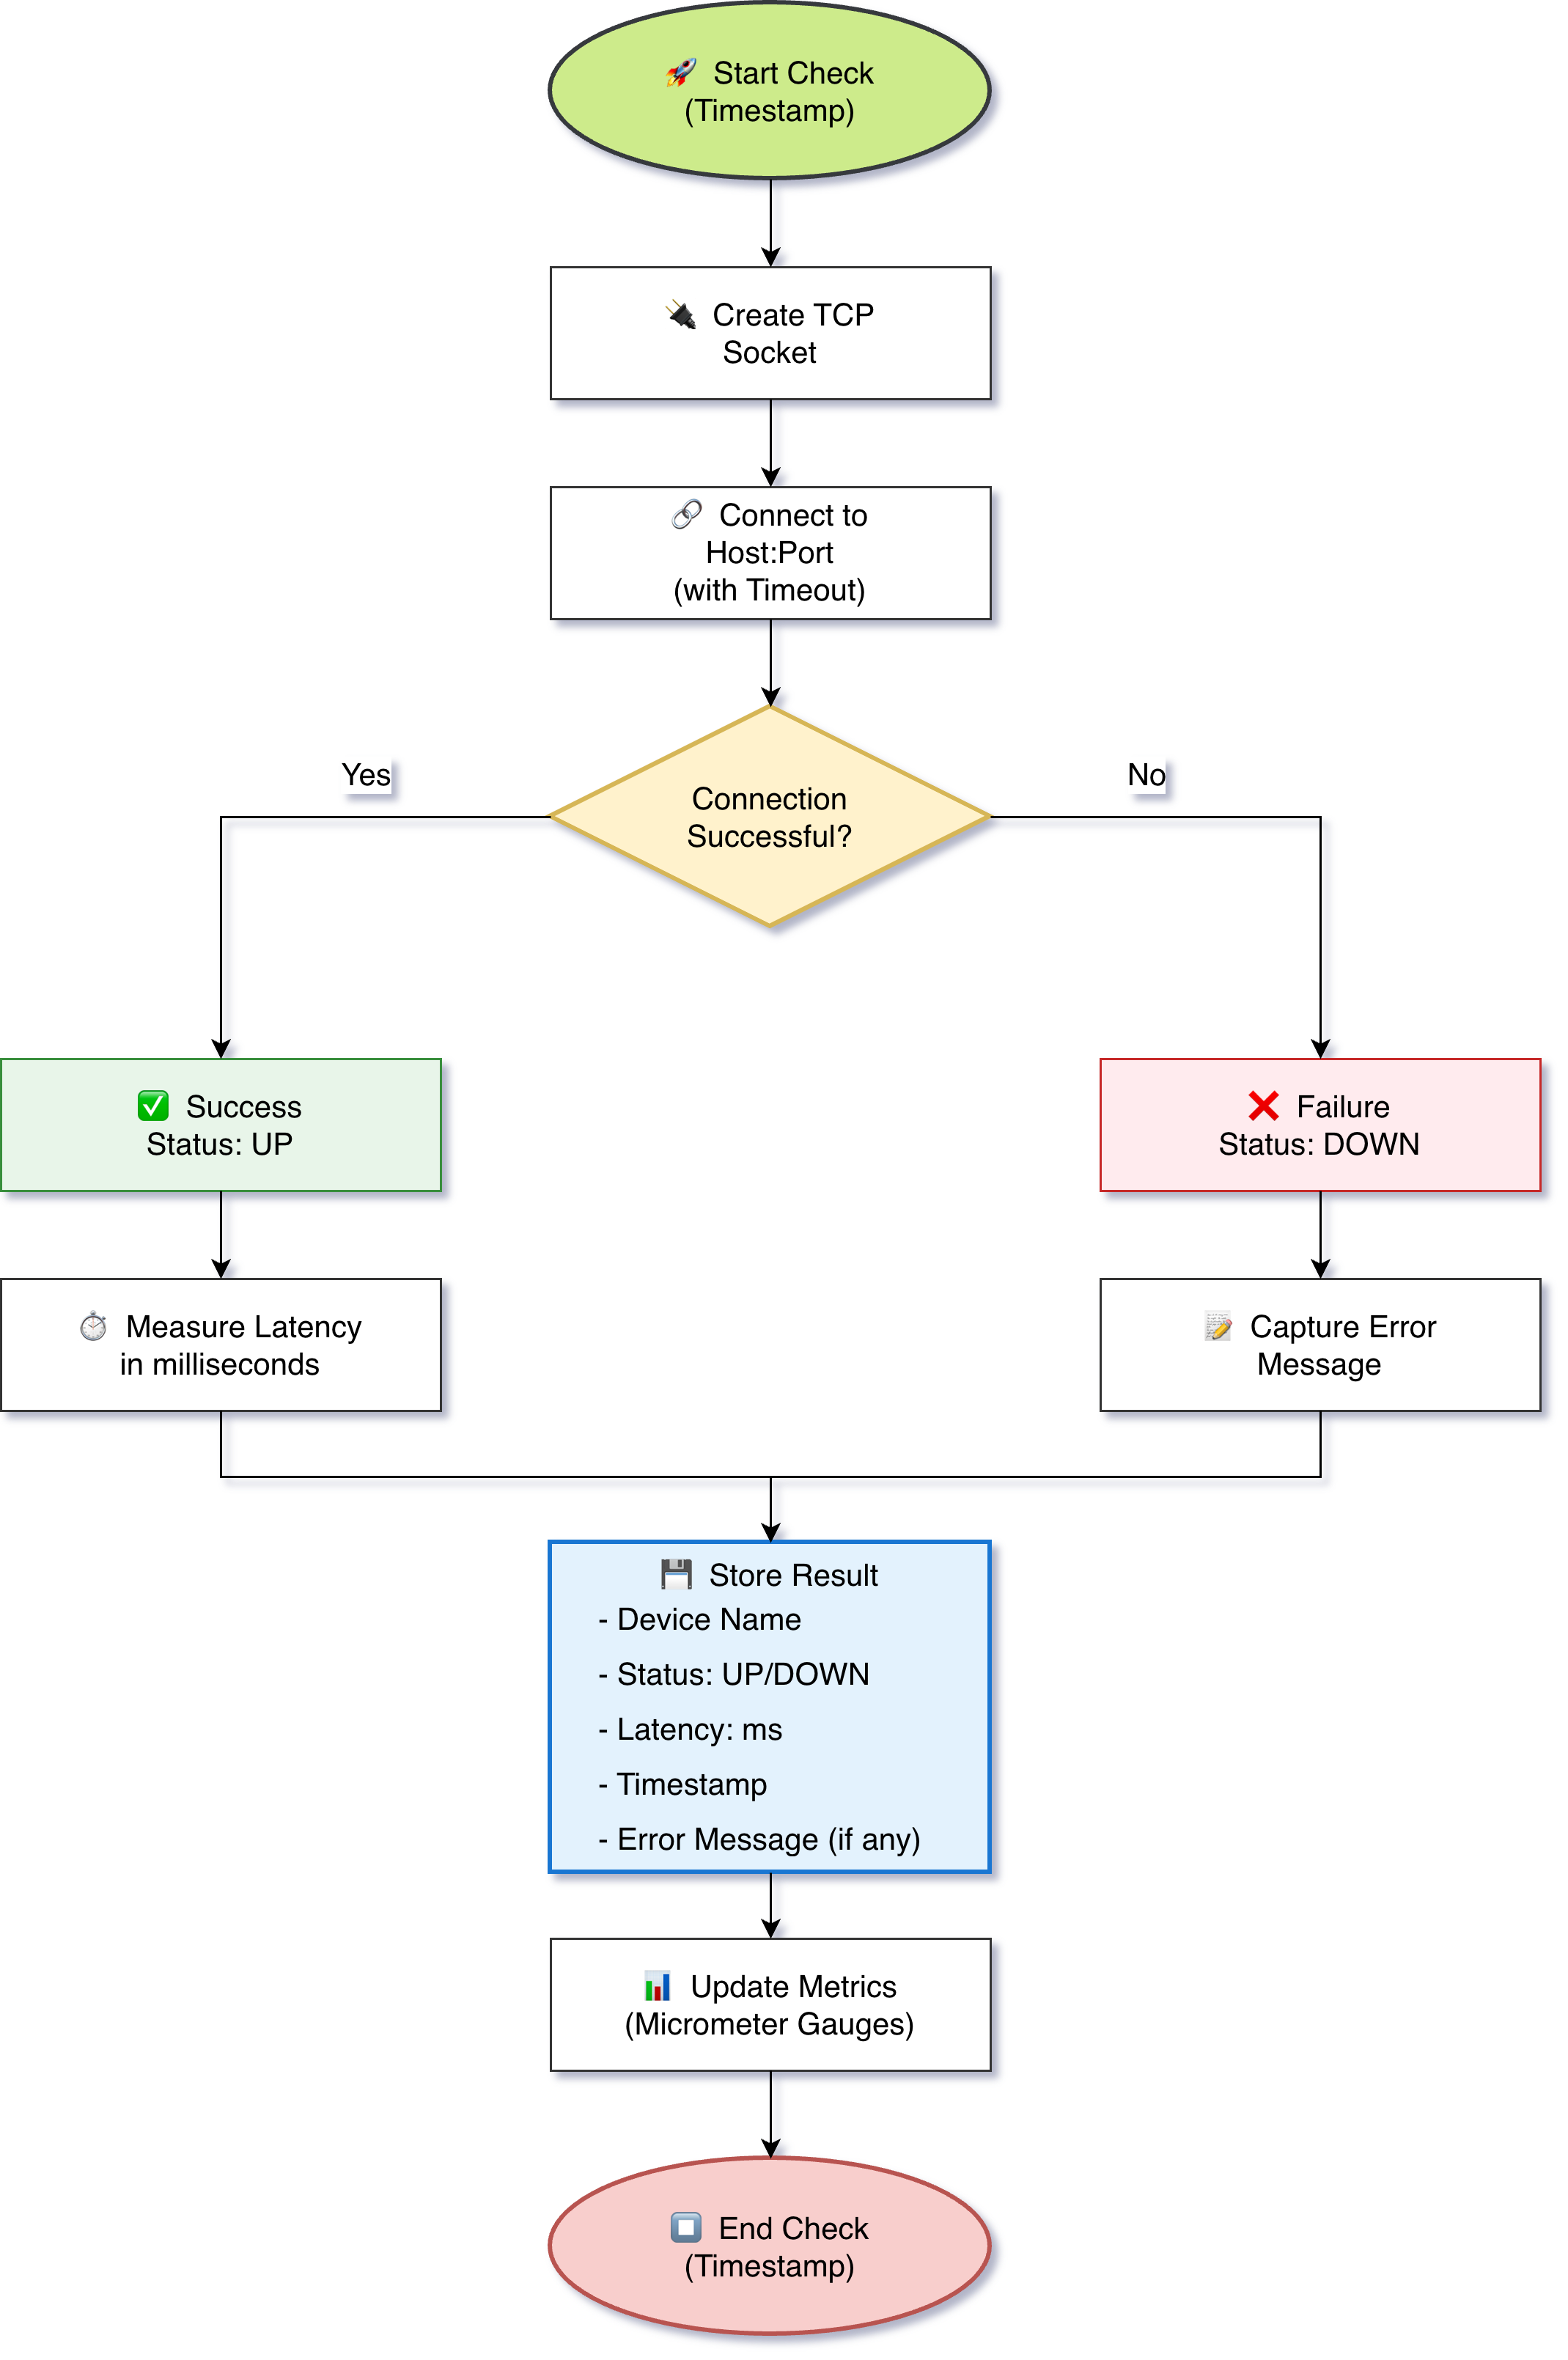
\includegraphics[width=0.6\textwidth]{Chapters/Graphics/pruefablauf.drawio.png}
\caption{Ablauf einer Erreichbarkeitsprüfung}
\label{fig:pruefablauf}
\end{figure}

Der Prüfungsablauf umfasst folgende Schritte:

\begin{enumerate}
    \item Start des Verbindungsversuchs mit Zeitstempel
    \item Versuch, eine TCP-Verbindung zum Ziel aufzubauen
    \item Bei Erfolg: Status auf \glqq erreichbar\grqq{} setzen und Latenz messen
    \item Bei Fehler: Status auf \glqq nicht erreichbar\grqq{} setzen und Fehlermeldung speichern
    \item Ende des Verbindungsversuchs mit Zeitstempel
    \item Speichern des Ergebnisses für Metrik-Export und REST-Schnittstelle
\end{enumerate}

Jedes Ziel wird unabhängig von den anderen Zielen geprüft. Der Ausfall eines einzelnen Ziels führt nicht zum Abbruch des gesamten Prüfzyklus (Anforderung N2).

\subsection{Fehlerbehandlung und Robustheit}
\label{subsec:fehlerbehandlung}

Die Fehlerbehandlung ist ein wesentlicher Bestandteil der Konzeption. Folgende Fehlerszenarien werden berücksichtigt:

\begin{itemize}
    \item \textbf{Zeitüberschreitung:} Wenn ein Ziel nicht innerhalb des konfigurierten Timeouts antwortet, wird die Verbindung abgebrochen und das Ziel als nicht erreichbar markiert.
    \item \textbf{Netzwerkfehler:} Bei Netzwerkproblemen (z.B. kein Route zum Ziel) wird der Fehler protokolliert und das Ziel als nicht erreichbar markiert.
    \item \textbf{Ungültige Konfiguration:} Bei fehlerhaften Konfigurationseinträgen (z.B. ungültige IP-Adresse) wird das Ziel übersprungen und ein Fehler protokolliert.
    \item \textbf{Ressourcenfehler:} Bei Erschöpfung von Systemressourcen (z.B. keine freien Sockets) wird der Prüfzyklus unterbrochen und ein Fehler protokolliert.
\end{itemize}

Durch diese Maßnahmen wird die Robustheit des Systems sichergestellt (Anforderung N2). Die Fehlerbehandlung folgt etablierten Patterns für robuste Systeme \cite{error-handling-patterns}.

\section{Konzeption des Metrik-Exports}
\label{sec:konzeption-metrik-export}

Der Metrik-Export stellt die Prüfergebnisse in einem standardisierten Format bereit, das von externen Monitoring-Systemen konsumiert werden kann.

\subsection{Metrikmodell}
\label{subsec:metrikmodell}

Für jedes Überwachungsziel werden zwei zentrale Metriken bereitgestellt:

\begin{itemize}
    \item \textbf{Status-Metrik:} Binärer Wert (1 für erreichbar, 0 für nicht erreichbar)
    \item \textbf{Latenz-Metrik:} Dauer des letzten Verbindungsversuchs in Millisekunden
\end{itemize}

Die Metriken werden mit Labels versehen, um die einzelnen Ziele zu unterscheiden. Vorgesehene Labels sind:

\begin{itemize}
    \item \textbf{Name:} Lesbarer Name des Ziels
    \item \textbf{Host:} Hostname oder IP-Adresse
    \item \textbf{Port:} Geprüfter TCP-Port
\end{itemize}

Zusätzlich werden Anwendungsmetriken bereitgestellt, die den Zustand des Monitoring-Dienstes selbst beschreiben (z.B. Anzahl der konfigurierten Ziele, Anzahl der aktiven Ziele, letzte Prüfungszeit).

\subsection{Exportformat}
\label{subsec:exportformat}

Das Exportformat orientiert sich an etablierten Standards für Metrik-Formate, insbesondere am Prometheus-Textformat \cite{prometheus-text-format}. Jede Metrik umfasst:

\begin{itemize}
    \item Metrik-Name
    \item Labels (in geschweiften Klammern)
    \item Numerischer Wert
    \item Optionaler Hilfstext (Beschreibung der Metrik)
\end{itemize}

Beispielhafte Darstellung:

\begin{lstlisting}[caption={Beispielhafte Darstellung einer Netzwerkmetrik},label={lst:metrikenbeispiel}]
# HELP network_device_up Current availability status
# TYPE network_device_up gauge
network_device_up{name="Router",host="192.0.2.1",port="443"} 1.0
network_device_latency_ms{name="Router",host="192.0.2.1",port="443"} 12.4
\end{lstlisting}

Das Format ermöglicht die einfache Integration mit Prometheus-kompatiblen Monitoring-Systemen (Anforderung F4).

\section{Konzeption der Zeitreihenspeicherung}
\label{sec:konzeption-zeitreihenspeicher}

Der Zeitreihenspeicher übernimmt die Persistierung der Metriken als Zeitreihen. Jede Metrik wird mit einem Zeitstempel versehen und in einer optimierten Datenbankstruktur gespeichert.

\subsection{Speichermodell}
\label{subsec:speichermodell}

Das Speichermodell umfasst folgende Entitäten:

\begin{itemize}
    \item \textbf{Metrik:} Name, Typ, Labels
    \item \textbf{Messwert:} Zeitstempel, numerischer Wert
    \item \textbf{Prüfergebnis:} Ziel, Status, Latenz, Prüfzeitpunkt, Fehlermeldung
    \item \textbf{Incident:} Alert-Informationen, Status, Zeitstempel
\end{itemize}

Die Speicherung als Zeitreihen ermöglicht die Auswertung aktueller und historischer Werte (Anforderung F5). Das Modell orientiert sich an etablierten Zeitreihen-Datenmodellen \cite{time-series-database-patterns}.

\subsection{Retentionspolitik}
\label{subsec:retentionspolitik}

Die Retentionspolitik definiert, wie lange Messwerte und Incidents gespeichert werden. Folgende Parameter sind konfigurierbar:

\begin{itemize}
    \item \textbf{Metrik-Retention:} Speicherdauer für Zeitreihendaten (z.B. 30 Tage)
    \item \textbf{Incident-Retention:} Speicherdauer für Incidents (z.B. 90 Tage)
\end{itemize}

Die Retentionspolitik ermöglicht einen Kompromiss zwischen Speichernutzung und Nachvollziehbarkeit (Anforderung N5, N6).

\section{Konzeption der Visualisierung}
\label{sec:konzeption-visualisierung}

Die Visualisierungskomponente stellt die gespeicherten Metriken und Incidents in Dashboards dar.

\subsection{Dashboard-Konzeption}
\label{subsec:dashboard-konzeption}

Das Dashboard umfasst folgende Bereiche:

\begin{itemize}
    \item \textbf{Übersicht:} Gesamtanzahl der Geräte, Online-Geräte, Offline-Geräte, aktive Incidents
    \item \textbf{Geräteliste:} Tabelle mit allen konfigurierten Zielen und deren aktuellem Status
    \item \textbf{Status-Panels:} Visuelle Darstellung des Erreichbarkeitsstatus (z.B. Ampelsystem)
    \item \textbf{Latenz-Zeitreihen:} Diagramme der TCP-Latenz über die Zeit
    \item \textbf{Incident-Historie:} Tabelle vergangener Störungen mit Dauer und Beschreibung
    \item \textbf{Anwendungsmetriken:} JVM-Metriken, Thread-Anzahl, Speichernutzung
\end{itemize}

Die Visualisierung ermöglicht einen schnellen operativen Überblick und die Analyse historischer Entwicklungen (Anforderung F6, N5). Die Dashboard-Gestaltung folgt etablierten Prinzipien der Informationsvisualisierung \cite{information-visualization-principles}.

\subsection{Alert-Visualisierung}
\label{subsec:alert-visualisierung}

Aktive Alerts werden in einem separaten Bereich dargestellt. Jeder Alert umfasst:

\begin{itemize}
    \item Alert-Name und Schweregrad
    \item Betroffenes Gerät
    \item Startzeitpunkt
    \item Beschreibung und Zusammenfassung
\end{itemize}

Die Darstellung erfolgt sortiert nach Schweregrad und Startzeitpunkt, um kritische Zustände priorisiert anzuzeigen.

\section{Konzeption der Alert-Komponente}
\label{sec:konzeption-alert}

Die Alert-Komponente erkennt kritische Zustände und leitet Benachrichtigungen weiter.

\subsection{Alert-Regeln}
\label{subsec:alert-regeln}

Alert-Regeln definieren Bedingungen, bei deren Erfüllung ein Alert ausgelöst wird. Folgende Regeltypen sind vorgesehen:

\begin{itemize}
    \item \textbf{Gerät nicht erreichbar:} Status-Metrik ist 0 für einen definierten Zeitraum (z.B. 30 Sekunden)
    \item \textbf{Latenz zu hoch:} Latenz-Metrik überschreitet einen definierten Grenzwert (z.B. 200\,ms) für einen definierten Zeitraum
    \item \textbf{Monitoring-Dienst nicht verfügbar:} Metrik-Endpunkt ist nicht erreichbar
\end{itemize}

Die Regeln werden kontinuierlich auf den gespeicherten Zeitreihen ausgewertet (Anforderung F7). Die Regeldefinition orientiert sich an etablierten Alerting-Konzepten \cite{alerting-best-practices}.

\subsection{Alert-Weiterleitung}
\label{subsec:alert-weiterleitung}

Bei Auslösung eines Alerts wird eine Benachrichtigung an den Incident-Speicher weitergeleitet. Die Weiterleitung umfasst:

\begin{itemize}
    \item Alert-Informationen (Name, Schweregrad, Labels, Annotations)
    \item Zeitstempel (Startzeitpunkt, optional Auflösungszeitpunkt)
    \item Status (Firing oder Resolved)
\end{itemize}

Die Alert-Weiterleitung erfolgt über einen Webhook-Endpunkt der REST-Schnittstelle.

\section{Konzeption des Incident-Speichers}
\label{sec:konzeption-incident-speicher}

Der Incident-Speicher übernimmt die persistente Speicherung von Alerts als Incidents.

\subsection{Incident-Modell}
\label{subsec:incident-modell}

Jedes Incident umfasst folgende Attribute:

\begin{itemize}
    \item \textbf{Identifikation:} Eindeutige ID und Alert-Fingerprint
    \item \textbf{Alert-Informationen:} Name, Schweregrad, Beschreibung
    \item \textbf{Betroffenes Gerät:} Name, Host, Port
    \item \textbf{Status:} Firing oder Resolved
    \item \textbf{Zeitstempel:} Startzeitpunkt und optional Auflösungszeitpunkt
    \item \textbf{Zusammenfassung und Beschreibung:} Kurz- und Langbeschreibung des Incidents
\end{itemize}

Das Incident-Modell ermöglicht die langfristige Nachverfolgung von Störungen (Anforderung F8). Das Modell orientiert sich an ITIL-basierten Incident-Management-Konzepten \cite{incident-management-itil}.

\subsection{Incident-Lifecycle}
\label{subsec:incident-lifecycle}

Der Lifecycle eines Incidents beschreibt die Verarbeitung eines durch das
Monitoring-System erkannten kritischen Zustands. Ausgangspunkt ist ein von
Alertmanager weitergeleiteter Alert mit dem Status \texttt{firing}. Um
doppelte Einträge zu vermeiden, wird zunächst der Fingerprint des eingehenden
Alerts geprüft. Der Fingerprint dient dabei zur eindeutigen Zuordnung
wiederholter Benachrichtigungen zu demselben Ereignis.

Existiert zu diesem Fingerprint noch kein aktives Incident, wird ein neuer
Incident-Datensatz angelegt und persistent gespeichert. Bereits vorhandene
aktive Incidents mit identischem Fingerprint werden bei weiteren
\texttt{firing}-Benachrichtigungen nicht erneut erstellt. Stattdessen bleibt
das vorhandene Incident im Status \texttt{FIRING}.

Der Lifecycle umfasst damit die folgenden Zustände und Verarbeitungsschritte:

\begin{enumerate}
    \item \textbf{Empfang eines Firing-Alerts:} Die Anwendung empfängt einen
    Alert mit dem Status \texttt{firing}.

    \item \textbf{Fingerprint-Prüfung:} Es wird geprüft, ob bereits ein aktives
    Incident mit demselben Fingerprint existiert.

    \item \textbf{Erstellung und Speicherung:} Falls kein aktives Incident
    vorhanden ist, wird ein neuer Incident-Datensatz mit Informationen zum
    Alert, zum betroffenen Gerät, zum Schweregrad und zum Startzeitpunkt
    erstellt und in der Datenbank gespeichert.

    \item \textbf{Aktiver Zustand:} Das Incident befindet sich im Status
    \texttt{FIRING}, solange der zugehörige Alert aktiv ist. Wiederholte
    \texttt{firing}-Alerts mit gleichem Fingerprint führen nicht zur Erstellung
    weiterer Incident-Datensätze.

    \item \textbf{Auflösung:} Beim Empfang eines Alerts mit dem Status
    \texttt{resolved} wird das zugehörige aktive Incident auf den Status
    \texttt{RESOLVED} gesetzt. Zusätzlich wird der Auflösungszeitpunkt
    gespeichert.
\end{enumerate}

Abbildung~\ref{fig:incident-lifecycle} zeigt den konzipierten Lifecycle eines
Incidents. Die optionale Archivierung oder Löschung aufgelöster Incidents nach
Ablauf einer Aufbewahrungsfrist ist als mögliche Erweiterung vorgesehen und
nicht Bestandteil des dargestellten Kernablaufs.

\begin{figure}[h]
\centering
% TODO: Lifecycle-Diagramm einfügen (z.B. als PDF oder PNG)
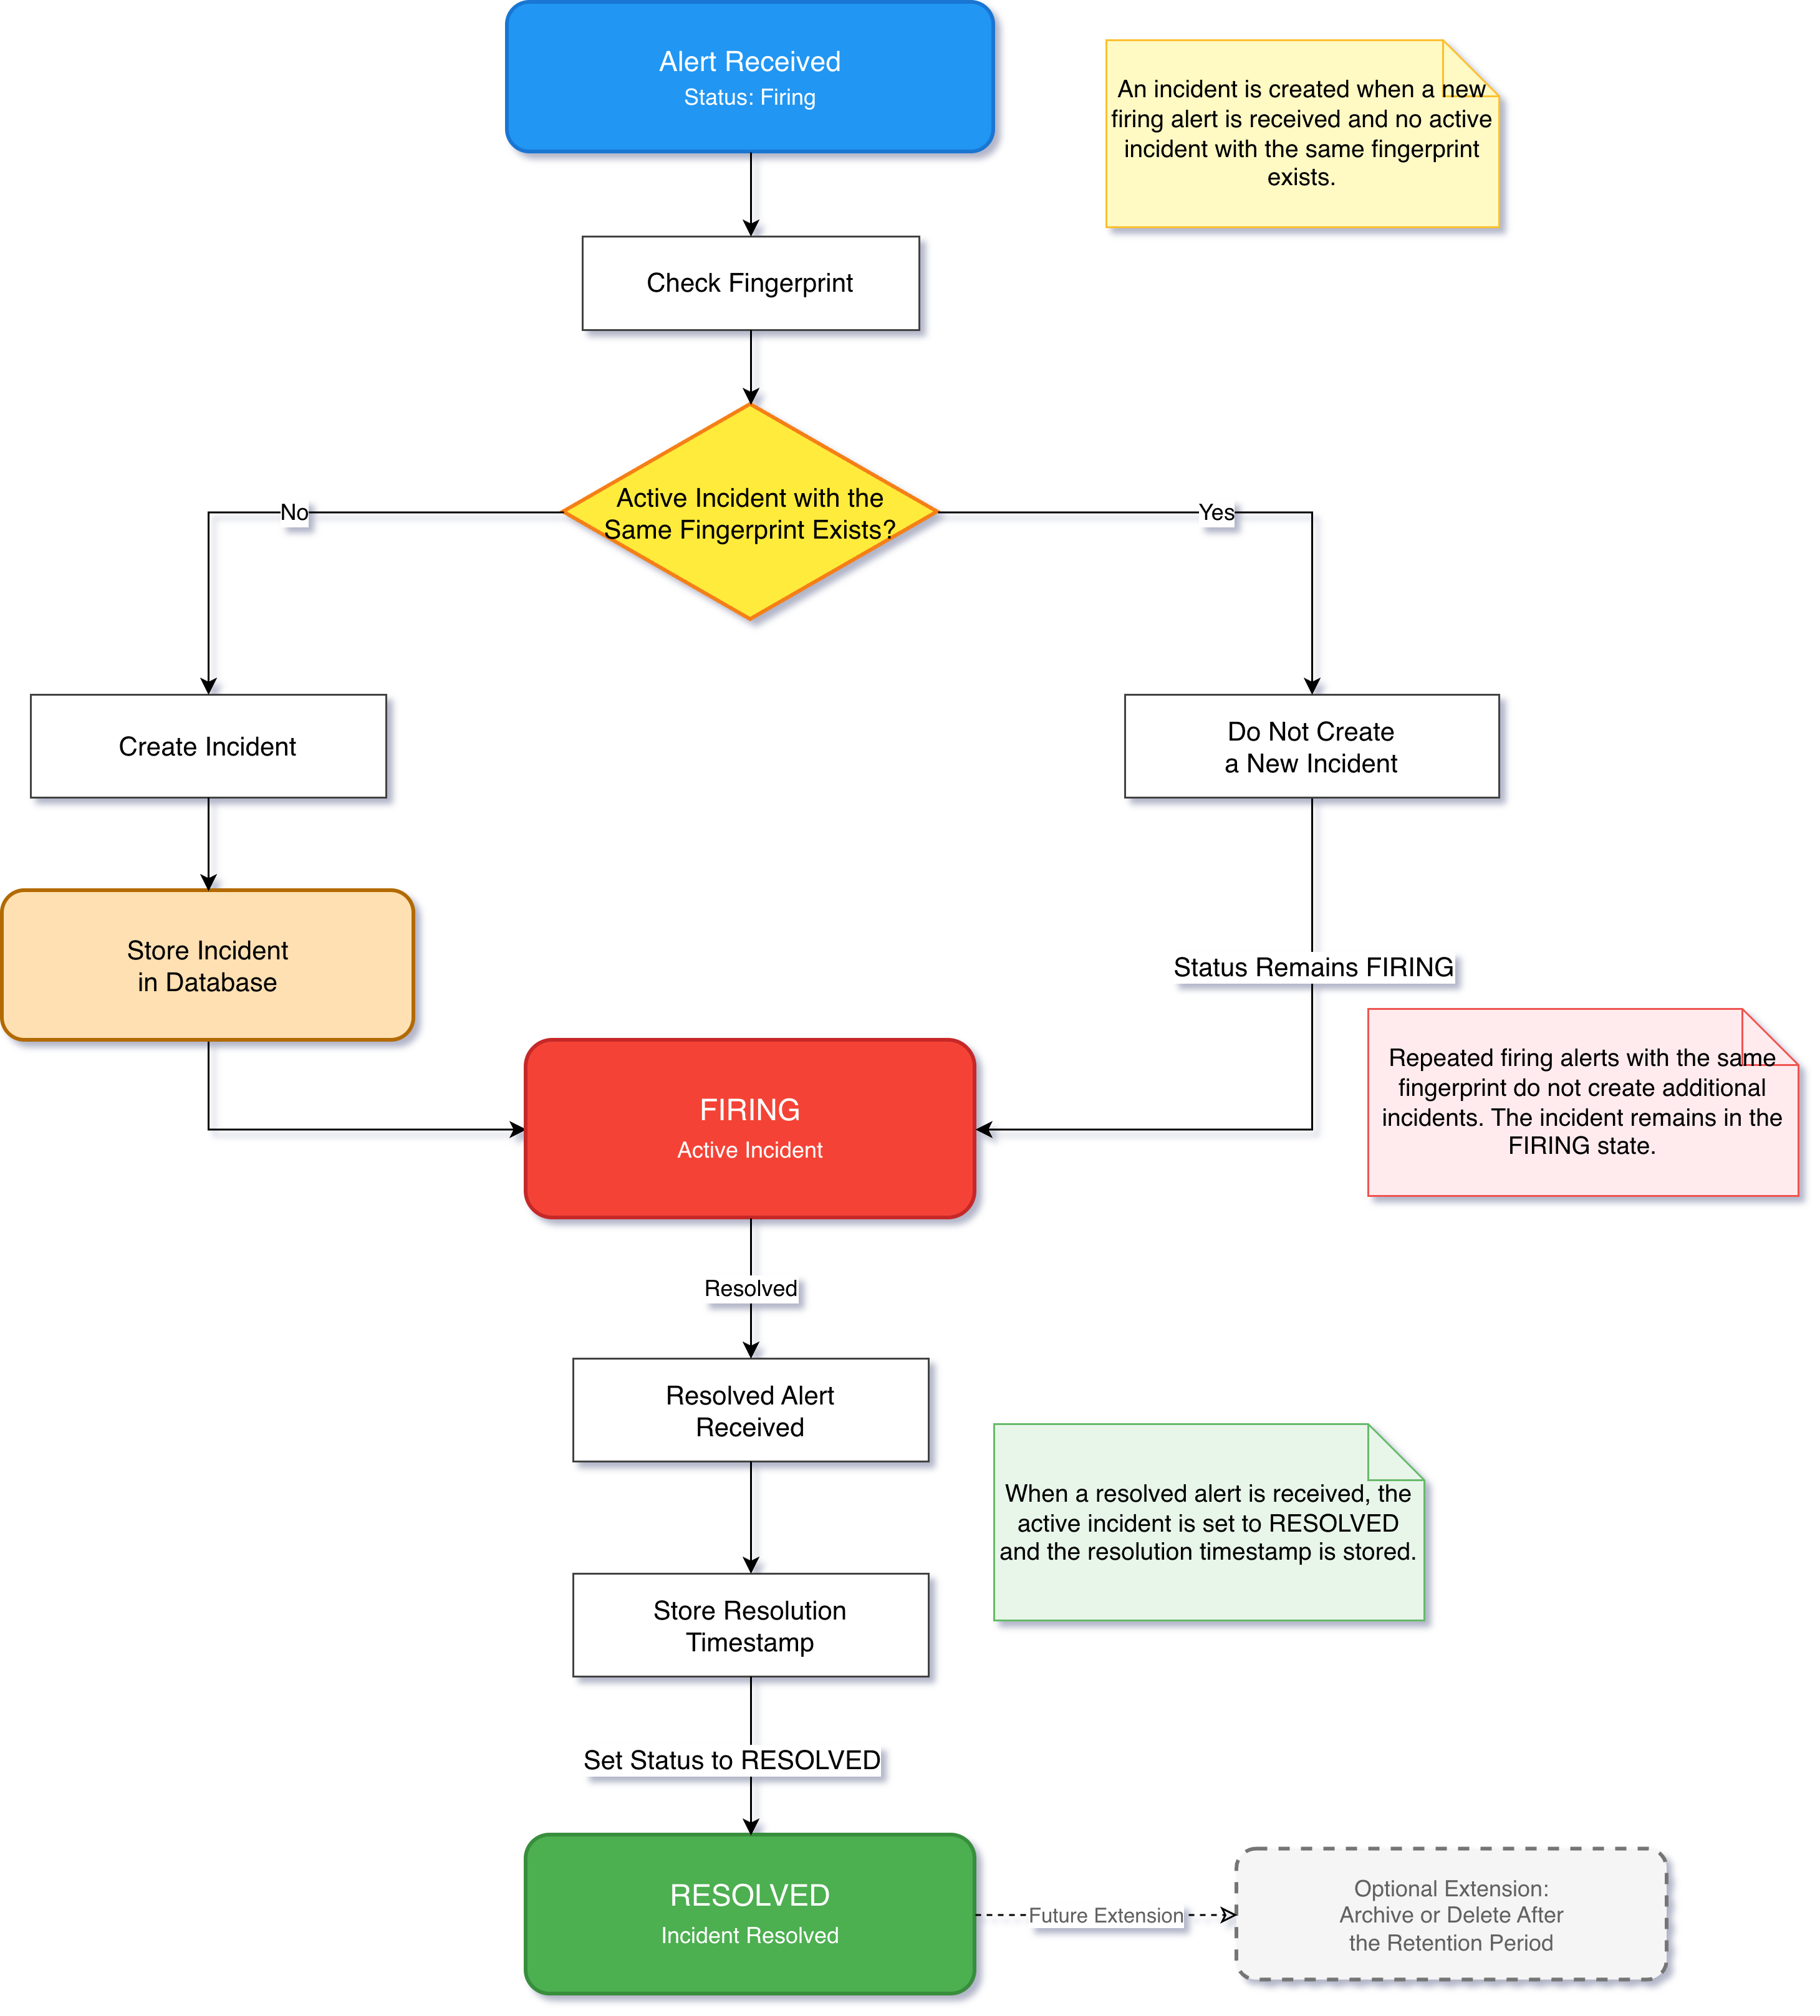
\includegraphics[width=0.7\textwidth]{Chapters/Graphics/incident-lifecycle.drawio.png}
\caption{Lifecycle eines Incidents}
\label{fig:incident-lifecycle}
\end{figure}

\section{Konzeption der REST-Schnittstelle}
\label{sec:konzeption-rest-schnittstelle}

Die REST-Schnittstelle ermöglicht die operative Abfrage von Konfiguration, Prüfergebnissen und Incidents.

\subsection{Endpunkte}
\label{subsec:endpunkte}

Die REST-Schnittstelle umfasst folgende Endpunkte:

\begin{itemize}
    \item \texttt{GET /api/status}: Dienststatus
    \item \texttt{GET /api/devices}: Liste der konfigurierten Geräte
    \item \texttt{GET /api/devices/\{name\}}: Einzelnes Gerät nach Name
    \item \texttt{GET /api/checks/latest}: Aktuelle Prüfergebnisse
    \item \texttt{GET /api/checks/history}: Historische Prüfergebnisse mit Filteroptionen
    \item \texttt{POST /api/checks/run}: Manuelle Auslösung eines Prüfzyklus
    \item \texttt{GET /api/incidents}: Alle Incidents
    \item \texttt{GET /api/incidents/active}: Aktive Incidents
    \item \texttt{GET /api/incidents/\{id\}}: Einzelnes Incident nach ID
    \item \texttt{POST /api/alerts}: Empfang von Alert-Webhooks
\end{itemize}

Die Endpunkte ermöglichen die Integration mit externen Systemen und die automatisierte Abfrage von Monitoring-Daten (Anforderung F9, F10). Die API-Design-Entscheidungen orientieren sich an den Prinzipien des REST-Architekturstils \cite{rest-architectural-style}.

\subsection{Sicherheit}
\label{subsec:sicherheit-rest}

Administrative Endpunkte (z.B. \texttt{POST /api/checks/run}, \texttt{POST /api/alerts}) werden durch Authentifizierung und Autorisierung geschützt. Folgende Sicherheitsmaßnahmen sind vorgesehen:

\begin{itemize}
    \item \textbf{HTTP Basic Authentication:} Benutzername und Passwort für administrative Zugriffe
    \item \textbf{Rollenbasierte Autorisierung:} Unterscheidung zwischen öffentlichen und administrativen Endpunkten
    \item \textbf{Externe Konfiguration der Credentials:} Speicherung der Zugangsdaten in Umgebungsvariablen, nicht im Quellcode
\end{itemize}

Diese Maßnahmen gewährleisten die Sicherheit der administrativen Endpunkte (Anforderung N7). Die Sicherheitskonzeption folgt etablierten Best Practices für API-Sicherheit \cite{api-security-best-practices}.

\section{Konzeption der containerisierten Bereitstellung}
\label{sec:konzeption-containerisierung}

Die gesamte Monitoring-Umgebung wird als containerisierte Anwendung bereitgestellt.

\subsection{Komponenten und Services}
\label{subsec:komponenten-services}

Die containerisierte Umgebung umfasst folgende Services:

\begin{itemize}
    \item \textbf{Monitoring-Dienst:} Spring-Boot-Anwendung mit Prüflogik und REST-API
    \item \textbf{Zeitreihenspeicher:} Prometheus-Container für Metrik-Speicherung
    \item \textbf{Visualisierung:} Grafana-Container für Dashboards
    \item \textbf{Alert-Komponente:} Alertmanager-Container für Alert-Verarbeitung
    \item \textbf{Demo-Service:} Optionaler NGINX-Container für Testzwecke
\end{itemize}

Alle Services werden über ein gemeinsames Docker-Netzwerk verbunden. Die Containerisierung folgt etablierten Best Practices für Docker-Anwendungen \cite{docker-best-practices}.

\subsection{Netzwerk und Volumes}
\label{subsec:netzwerk-volumes}

Die Konzeption umfasst:

\begin{itemize}
    \item \textbf{Docker-Netzwerk:} Ermöglicht die Kommunikation der Services über ihre Servicenamen
    \item \textbf{Persistente Volumes:} Speicherung von Zeitreihendaten, Incident-Daten und Dashboard-Konfigurationen
    \item \textbf{Konfigurations-Volumes:} Einbinden von Konfigurationsdateien in die Container
\end{itemize}

Diese Konzeption ermöglicht eine reproduzierbare Bereitstellung (Anforderung N3). Die Volume-Konzeption orientiert sich an etablierten Patterns für persistente Daten in Containern \cite{docker-volume-patterns}.

\section{Zusammenfassung}
\label{sec:zusammenfassung-konzeption}

Die Konzeption beschreibt eine modulare, technologieunabhängige Architektur für ein leichtgewichtiges Netzwerk-Monitoring-System. Die entwickelten Lösungsansätze schließen die in Kapitel~\ref{ch:analyse} identifizierten Lücken bestehender Monitoring-Lösungen und erfüllen die ermittelten Anforderungen.

Die zentralen Konzepte umfassen:

\begin{itemize}
    \item \textbf{Modulare Architektur:} Trennung der Verantwortlichkeiten auf mehrere Komponenten
    \item \textbf{Incident-Historie:} Persistente Speicherung von Alerts zur langfristigen Nachverfolgung
    \item \textbf{REST-Schnittstelle:} Umfassende API für operative Abfragen
    \item \textbf{Containerisierung:} Reproduzierbare Bereitstellung mit Docker Compose
    \item \textbf{Leichtgewichtigkeit:} Fokus auf Kernfunktionen ohne Überdimensionierung
    \item \textbf{Robustheit:} Fehlerbehandlung und unabhängige Prüfung einzelner Ziele
\end{itemize}

Die Konzeption bildet die Grundlage für die Implementierung in Kapitel~\ref{ch:implementierung}. Die beschriebenen Konzepte sind technologieunabhängig formuliert, können jedoch direkt mit konkreten Technologien wie Java, Spring Boot, Prometheus, Grafana und Docker umgesetzt werden.